\documentclass[12pt,a4paper]{scrartcl} 
\usepackage[utf8]{inputenc}
\usepackage[english,russian]{babel}
\usepackage{indentfirst}
\usepackage{misccorr}
\usepackage{graphicx}
\usepackage{amsmath}

\begin{document}

\begin{titlepage}
		\begin{center}
			\large
			МИНИСТЕРСТВО НАУКИ И ВЫСШЕГО ОБРАЗОВАНИЯ РОССИЙСКОЙ ФЕДЕРАЦИИ
			
			Федеральное государственное бюджетное образовательное учреждение высшего образования
			
			\textbf{АДЫГЕЙСКИЙ ГОСУДАРСТВЕННЫЙ УНИВЕРСИТЕТ}
			\vspace{0.25cm}
			
			Инженерно-физический факультет
			
			Кафедра автоматизированных систем обработки информации и управления
			\vfill

			\vfill
			
			\textsc{Отчет по практике}\\[5mm]
			
			{\LARGE \textit{Обход графа в глубину}}
			\bigskip
			
			1 курс, группа 1УТС
		\end{center}
		\vfill
		
		\newlength{\ML}
		\settowidth{\ML}{«\underline{\hspace{0.7cm}}» \underline{\hspace{2cm}}}
		\hfill\begin{minipage}{0.5\textwidth}
			Выполнил:\\
			\underline{\hspace{\ML}} К.\,А.~Кузьмин\\
			«\underline{\hspace{0.7cm}}» \underline{\hspace{2cm}} 2021 г.
		\end{minipage}%
		\bigskip
		
		\hfill\begin{minipage}{0.5\textwidth}
			Руководитель:\\
			\underline{\hspace{\ML}} С.\,В.~Теплоухов\\
			«\underline{\hspace{0.7cm}}» \underline{\hspace{2cm}} 2021 г.
		\end{minipage}%
		\vfill
		
		\begin{center}
			Майкоп, 2021 г.
		\end{center}
	\end{titlepage}

\section{Введение}
\label{sec:intro}

\begin{enumerate}
 \item Текстовая формулировка задачи:

Написать приложение для обхода графа в глубину.
 \item Пример кода, решающего данную задачу:

Пример приведен в пункте ~\ref{sec:exp} на стр.~\pageref{sec:exp}.
 \item График:

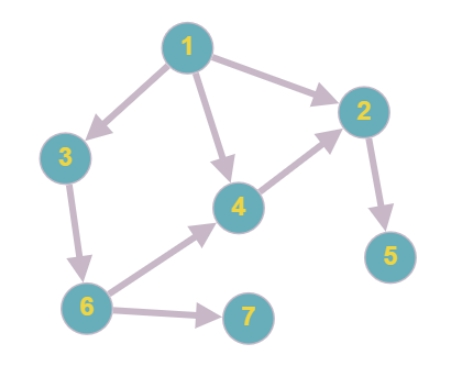
\includegraphics[width=0.4\textwidth]{graph.jpg}
 \item Скриншот программы:

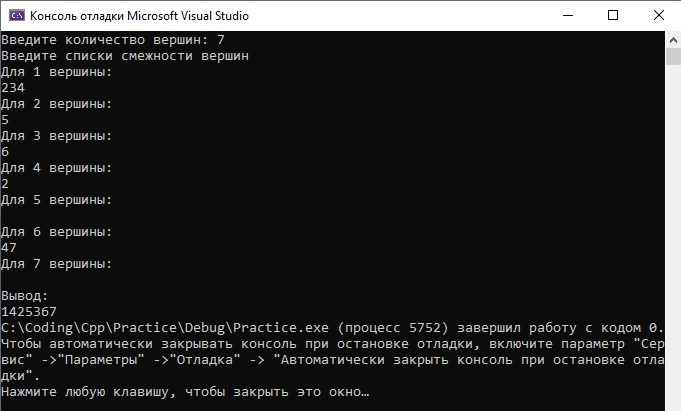
\includegraphics[width=0.6\textwidth]{screen.jpg}

\end{enumerate}

\section{Ход работы}
\label{sec:exp}
\subsection{Код приложения}
\label{sec:exp:code}
\begin{verbatim}

#include <iostream>
#include <string>
#include <stack>
#include <limits>
using namespace std;

int main()
{
    setlocale(LC_ALL, "rus");
    short int n;
    int mas[7][7];
    string input[7];
    do
    {
        cout << "Введите количество вершин: ";
        cin >> n;
    }
    while ((n < 2) || (n > 7));
    cout << "Введите списки смежности вершин" << endl;
    cin.ignore(numeric_limits<streamsize>::max(), '\n');
    for (int i = 0; i < n; i++)
    {
        cout << "Для " << i + 1 << " вершины:" << endl;
        getline(cin, input[i]);
        for (int j = 0; j < input[i].length(); j++)
        {
            if (input[i][j] == ' ')
            {
                input[i].erase(j, 1);
                j--;
            }
        }
    }
    for (int i = 0; i < n; i++)
    {
        for (int j = 0; j < n; j++)
        {
            mas[i][j] = 0;
        }
    }
    for (int i = 0; i < n; i++)
    {
        for (int j = 0; j < input[i].length(); j++)
        {
            mas[i][static_cast<int>(input[i][j]) - 48 - 1] = 1;
        }
    }
    cout << "Вывод:" << endl;
    stack <int> Stack;
    int nodes[7];
    for (int i = 0; i < n; i++) nodes[i] = 0;
    Stack.push(0);
    while (!Stack.empty())
    {
        int node = Stack.top();
        Stack.pop();
        if (nodes[node] == 2) continue;
        nodes[node] = 2;
        for (int j = 0; j < n; j++)
        {
            if (mas[node][j] == 1 && nodes[j] != 2)
            {
                Stack.push(j);
                nodes[j] = 1;
            }
        }
        cout << node + 1;
    }
    return 0;
}

\end{verbatim}

\section{Пример вставки изображения}
\label{sec:picexample}
\begin{figure}[h]
	\centering
	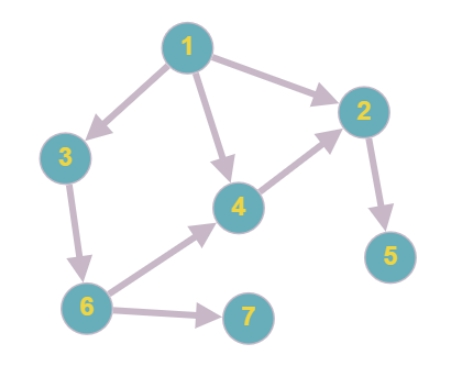
\includegraphics[width=0.4\textwidth]{graph.jpg}
	\caption{Граф}\label{fig:graph}
\end{figure}

Пример графа представлен на рис. ~\ref{fig:graph}.

\section{Пример библиографических ссылок}

Для изучения «внутренностей» \TeX{} необходимо 
изучить~\cite{Knuth-2003}, а для использования \LaTeX{} лучше
почитать~\cite{Lvovsky-2003, Voroncov-2005}.

\begin{thebibliography}{9}
\bibitem{Knuth-2003}Кнут Д.Э. Всё про \TeX. \newblock --- Москва: Изд. Вильямс, 2003 г. 550~с.
\bibitem{Lvovsky-2003}Львовский С.М. Набор и верстка в системе \LaTeX{}. \newblock --- 3-е издание, исправленное и дополненное, 2003 г.
\bibitem{Voroncov-2005}Воронцов К.В. \LaTeX{} в примерах. 2005 г.
\end{thebibliography}

\end{document}